%%%%%%%%%%%%%%%%%%%%%%%%%%%%%%%%%%%%%%%%%%%%%%%%%%%%%%%%%%%%%%%%%%%%%%%%%%%%%%%%
\chapter{Постановка задачи и выбор пути решения}
%%%%%%%%%%%%%%%%%%%%%%%%%%%%%%%%%%%%%%%%%%%%%%%%%%%%%%%%%%%%%%%%%%%%%%%%%%%%%%%%

В данном разделе рассматриваются основные требования, предъявляемые к методу обнаружения клонов. Приводится постановка и подробное описание задач, решаемых в рамках данной работы, в том числе:
\begin{itemize}
\setlength\itemsep{0mm}
\item задача разработки метода обнаружения клонов, основанного на использовании искусственных нейронных сетей
\item задача разработки прототипа инструмента обнаружения
\end{itemize}
%%%%%%%%%%%%%%%%%%%%%%%%%%%%%%%%%%%%%%%%%%%%%%%%%%%%%%%%%%%%%%%%%%%%%%%%%%%%%%%%
\section{Задача разработки интеллектуального метода обнаружения клонов}
%%%%%%%%%%%%%%%%%%%%%%%%%%%%%%%%%%%%%%%%%%%%%%%%%%%%%%%%%%%%%%%%%%%%%%%%%%%%%%%%

Целью данной работы является разработка метода для обнаружения клонов. Главное требование, которое предъявляется к разрабатываемому методу - использование искусственных нейронных сетей. Кроме того, разрабатываемый метод интеллектуального обнаружения клонов должен обеспечивать решение следующих задач:
\begin{itemize}
\setlength\itemsep{0mm}
\item обнаружение клонов I-III типов;
\item максимизация полноты и точности обнаружения;
\item извлечение информации о клонах в виде клоновых классов.
\end{itemize}

Несмотря на тот факт, что разрабатываемый метод должен быть интеллектуальным, в качестве предварительной обработки необходимо привести исходный код к одному из подходящих видов внутреннего представления. В предлагаемом подходе было решено использовать несколько представлений (гибридный метод). Этими представлениями являются AST и последовательность токенов. 

Использование AST позволяет сохранить информацию о структуре исходного текста программы, именно благодаря этому становится возможным увеличить полноту и точность результатов.

Использование токенов в качестве представления исходного кода позволяет, в свою очередь, значительно сократить размер входных данных.

Общую структуру внутреннего представления кода можно увидеть на рис.~\ref{fig:stages}

\begin{figure}[htbp]
\centering
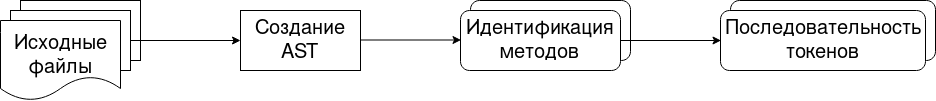
\includegraphics[width=\textwidth]{stages.png}
\caption{Предлагаемый метод обнаружения клонов}
\label{fig:stages}
\end{figure}
